\chapter{Results Comparison}
\label{ch:results}
In this chapter, we are going to compare the results obtained after running the
tests. Then we give a description of some hard cases that the presented
algorithms fail to solve and we conclude with a brief description of how they
may be addressed.
%
%
%
\section{Results}
We created 300 random tests with different values of number of nodes, number of
agents, number of goals and connection density, taken from:
\begin{minted}[linenos=false]{python}
agents_occ = [5, 10, 20, 50, 75]  # Percentages of agents w.r.t. #nodes
nodes = [10, 20, 50, 100]         # Number of nodes in the scenario
n_goals = [1, 2, 5, 10, 20, 50]   # Number of goals in the scenario
p_conn = [0.1, 0.25, 0.5]         # Probability that an edge between two nodes exists
\end{minted}
The specifics of the computer used to run the tests are the following:
\begin{itemize}
  \item Processor: AMD Ryzen 3700X;
  \item RAM: 32GB 3600MT/s;
  \item Operating system: Arch Linux with Linux Kernel 5.18.8;
  \item CPLEX version 22.1.0;
  \item C++ compiler: \texttt{gcc} version 12.1.0, code compiled with standard
    C++17.
\end{itemize}
The tests were then run multiple times to ensure the reliability of the data
collected. Each test was run with the different versions of the algorithms:
\begin{itemize}
  \item \milc{CBS_TDSP_MKS}: \acrs{CBS} with \acrs{TDSP} for the low-level
    search and makespan for the objective function;
  \item \milc{CBS_TDSP_SIC}: \acrs{CBS} with \acrs{TDSP} for the low-level
    search and \acrs{SIC} for the objective function;
  \item \milc{CBS_ST_MKS}: \acrs{CBS} with spanning trees for the 
    low-level search and makespan for the objective function;
  \item \milc{CBS_ST_SIC}: \acrs{CBS} with spanning trees for the
    low-level search and \acrs{SIC} for the objective function;
  \item \milc{CP_MKS}: \acrl{cp} minimizing the makespan;
  \item \milc{CP_SIC}: \acrl{cp} minimizing the \acrs{SIC};
\end{itemize}
Also, the executions were sequentialized through Python using the
\texttt{subproces} module and, to avoid infinite loops when it is not possible
to find a solution, we used the Unix \texttt{timeout} system call to kill the
program after a certain amount of time. We used three different periods of time
for the timeout in order to test whether some tests would require only more
time or if they could not be solved. We have actually noticed an increment in
the solved tests as it is possible to see from Table~\ref{tab:randomTests}.
In particular, we noticed that the constraint programming approach requires a
lot of time to solve its inputs and this actually agrees with the findings of
other authors~\cite{MAPF_overview}. \newline
It is worth noticing that the majority of the cases in which \acrs{CT} fails is
due to the long computational times. Indeed, \acrs{CT} basically tries to find
all the possible solutions that are valid with the given constraints and that
minimize the objective function. The problem though is combinatorial in the
number of decision variables and hence at each incremented step, it becomes
more and more demanding to complete. 
\newcolumntype{?}{!{\vrule width 1.5pt}}
\newcommand{\mc}[3]{\multicolumn{#1}{#2}{#3}} 
\begin{table}[htpb]
  \centering
  \caption{The results of the program when faced with 300 random tests of
  increasing difficulty.}
  \label{tab:randomTests}

  \begin{tabular}{l?c|c|c?c|c|c}
                & \mc{3}{c?}{Test completed} & \mc{3}{c}{Average run time [ms]} \\
    \Xhline{1.5pt}
    \diagbox[linewidth=1.5pt]{Program}{Timeout} & \mc{1}{c}{1s} & \mc{1}{c}{10s} & \mc{1}{c?}{60s} & \mc{1}{c}{1s} & \mc{1}{c}{10s} & \mc{1}{c}{60s} \\
    \Xhline{1.5pt}
    \milc{CBS_TDSP_MKS} & 187 & 189 & 189 & 15.86  & 39.93   & 40.51   \\ 
    \milc{CBS_TDSP_SIC} & 184 & 185 & 185 & 13.32  & 59.78   & 56.98   \\
    \milc{CBS_ST_MKS}   & 30  & 34  & 35  & 24.26  & 398.02  & 1459.09  \\
    \milc{CBS_ST_SIC}   & 27  & 28  & 29  & 37.45  & 123.25  & 381.41  \\
    \milc{CP_MKS}       & 21  & 36  & 36  & 362.09 & 2086.08 & 2234.65 \\
    \milc{CP_SIC}       & 17  & 28  & 28  & 273.51 & 1594.02 & 1501.23 
  \end{tabular}
\end{table}\newline
The warehouse results are show from Table~\ref{tab:mag12} to 
Table~\ref{tab:mag2_2_2}. What appears evident is that the algorithm 
\acrs{TDSP} presented in Section~\ref{ssec:tdsp} is the one that is able to
solve the most number of tests out of all the others and especially in the
lowest time possible. \newline
Moreover, we see that \acrs{CP} takes a lot of time to compute a feasible
solution, and it also needs a lot of memory, albeit not reported in the tables
due to difficulties in accurately stating the memory consumption. \newline
\begin{table}[htpb]
  \centering
  \caption{The results for the \milc{MAG12} map over which 25 scenarios were
    tested with different numbers of goals and agents.}
  \label{tab:mag12}
  \begin{tabular}{l?c|c|c?c|c|c}
                & \mc{3}{c?}{Test completed} & \mc{3}{c}{Average run time [ms]} \\
    \Xhline{1.5pt}
    \diagbox[linewidth=1.5pt]{Program}{Timeout} & \mc{1}{c}{1s} & \mc{1}{c}{10s} & \mc{1}{c?}{60s} & \mc{1}{c}{1s} & \mc{1}{c}{10s} & \mc{1}{c}{60s} \\
    \Xhline{1.5pt}
    \milc{CBS_TDSP_MKS} & 12 & 15 & 16 & 207.87 & 950.47 & 1857.94 \\ 
    \milc{CBS_TDSP_SIC} & 12 & 14 & 15 & 208.28 & 524.43 & 1529.46 \\
    \milc{CBS_ST_MKS}   & 0  & 0  & 0  & --     & --     & --      \\
    \milc{CBS_ST_SIC}   & 0  & 0  & 0  & --     & --     & --      \\
    \milc{CP_MKS}       & 0  & 0  & 0  & --     & --     & --      \\
    \milc{CP_SIC}       & 0  & 0  & 0  & --     & --     & --      
  \end{tabular}
\end{table}
\begin{table}[htpb]
  \centering
  \caption{The results for the \milc{MAG1} map over which 20 scenarios were
    tested with different numbers of goals and agents.}
  \label{tab:mag11}
  \begin{tabular}{l?c|c|c?c|c|c}
                & \mc{3}{c?}{Test completed} & \mc{3}{c}{Average run time [ms]} \\
    \Xhline{1.5pt}
    \diagbox[linewidth=1.5pt]{Program}{Timeout} & \mc{1}{c}{1s} & \mc{1}{c}{10s} & \mc{1}{c?}{60s} & \mc{1}{c}{1s} & \mc{1}{c}{10s} & \mc{1}{c}{60s} \\
    \Xhline{1.5pt}
    \milc{CBS_TDSP_MKS} & 13 & 13 & 13 & 117.59 & 118.13 & 117.43 \\ 
    \milc{CBS_TDSP_SIC} & 12 & 12 & 12 & 124.19 & 124.25 & 125.51 \\
    \milc{CBS_ST_MKS}   & 0  & 0  & 0  & --     & --     & --     \\
    \milc{CBS_ST_SIC}   & 0  & 0  & 0  & --     & --     & --     \\
    \milc{CP_MKS}       & 0  & 0  & 0  & --     & --     & --     \\
    \milc{CP_SIC}       & 0  & 0  & 0  & --     & --     & --     
  \end{tabular}
\end{table}
\begin{table}[htpb]
  \centering
  \caption{The results for the \milc{MAG2} map over which 20 scenarios were
    tested with different numbers of goals and agents.}
  \label{tab:mag2}
  \begin{tabular}{l?c|c|c?c|c|c}
                & \mc{3}{c?}{Test completed} & \mc{3}{c}{Average run time [ms]} \\
    \Xhline{1.5pt}
    \diagbox[linewidth=1.5pt]{Program}{Timeout} & \mc{1}{c}{1s} & \mc{1}{c}{10s} & \mc{1}{c?}{60s} & \mc{1}{c}{1s} & \mc{1}{c}{10s} & \mc{1}{c}{60s} \\
    \Xhline{1.5pt}
    \milc{CBS_TDSP_MKS} & 10 & 11 & 11 & 72.78 & 263.56 & 262.04 \\ 
    \milc{CBS_TDSP_SIC} & 10 & 11 & 11 & 73.07 & 185.24 & 186.90 \\
    \milc{CBS_ST_MKS}   & 0  & 0  & 0  & --    & --     & --     \\
    \milc{CBS_ST_SIC}   & 0  & 0  & 0  & --    & --     & --     \\
    \milc{CP_MKS}       & 0  & 0  & 0  & --    & --     & --     \\
    \milc{CP_SIC}       & 0  & 0  & 0  & --    & --     & --     
  \end{tabular}
\end{table}
\begin{table}[htpb]
  \centering
  \caption{The results for the \milc{MAG2_1} map over which 20 scenarios were
    tested with different numbers of goals and agents.}
  \label{tab:mag2_1}

  \begin{tabular}{l?c|c|c?c|c|c}
                & \mc{3}{c?}{Test completed} & \mc{3}{c}{Average run time [ms]} \\
    \Xhline{1.5pt}
    \diagbox[linewidth=1.5pt]{Program}{Timeout} & \mc{1}{c}{1s} & \mc{1}{c}{10s} & \mc{1}{c?}{60s} & \mc{1}{c}{1s} & \mc{1}{c}{10s} & \mc{1}{c}{60s} \\
    \Xhline{1.5pt}
    \milc{CBS_TDSP_MKS} & 9 & 9 & 9 & 27.53 & 27.9 & 28.13 \\ 
    \milc{CBS_TDSP_SIC} & 9 & 9 & 9 & 27.43 & 27.6 & 27.63 \\
    \milc{CBS_ST_MKS}   & 1 & 1 & 1 &  0.55 & 0.56 &  0.56 \\
    \milc{CBS_ST_SIC}   & 1 & 1 & 1 &  0.96 & 0.55 &  0.96 \\
    \milc{CP_MKS}       & 0 & 0 & 0 & --    & --   &  --   \\
    \milc{CP_SIC}       & 0 & 0 & 0 & --    & --   &  -- 
  \end{tabular}
\end{table}
\begin{table}[htpb]
  \centering
  \caption{The results for the \milc{MAG2_2} map over which 20 scenarios were
    tested with different numbers of goals and agents.}
  \label{tab:mag2_2}

  \begin{tabular}{l?c|c|c?c|c|c}
                & \mc{3}{c?}{Test completed} & \mc{3}{c}{Average run time [ms]} \\
    \Xhline{1.5pt}
    \diagbox[linewidth=1.5pt]{Program}{Timeout} & \mc{1}{c}{1s} & \mc{1}{c}{10s} & \mc{1}{c?}{60s} & \mc{1}{c}{1s} & \mc{1}{c}{10s} & \mc{1}{c}{60s} \\
    \Xhline{1.5pt}
    \milc{CBS_TDSP_MKS} & 13 & 13 & 13 &  7.50 &  7.54 &     7.49 \\ 
    \milc{CBS_TDSP_SIC} & 14 & 14 & 14 & 32.93 & 32.73 &    32.67 \\
    \milc{CBS_ST_MKS}   & 1  & 1  & 1  &  4.57 &  4.58 &     4.57 \\
    \milc{CBS_ST_SIC}   & 2  & 2  & 2  & 43.00 & 42.74 &    42.74 \\
    \milc{CP_MKS}       & 0  & 0  & 1  & --    & --    & 47782.30 \\
    \milc{CP_SIC}       & 0  & 0  & 0  & --    & --    & --
  \end{tabular}
\end{table}
\begin{table}[htpb]
  \centering
  \caption{The results for the \milc{MAG2_1_1} map over which 15 scenarios were
    tested with different numbers of goals and agents.}
  \label{tab:mag2_1_1}

  \begin{tabular}{l?c|c|c?c|c|c}
                & \mc{3}{c?}{Test completed} & \mc{3}{c}{Average run time [ms]} \\
    \Xhline{1.5pt}
    \diagbox[linewidth=1.5pt]{Program}{Timeout} & \mc{1}{c}{1s} & \mc{1}{c}{10s} & \mc{1}{c?}{60s} & \mc{1}{c}{1s} & \mc{1}{c}{10s} & \mc{1}{c}{60s} \\
    \Xhline{1.5pt}
    \milc{CBS_TDSP_MKS} & 7 & 7 & 7 & 8.13 &  8.08 & 8.26 \\ 
    \milc{CBS_TDSP_SIC} & 7 & 7 & 7 & 7.32 &  7.59 & 7.28 \\
    \milc{CBS_ST_MKS}   & 2 & 2 & 2 & 9.21 & 10.28 & 9.13 \\
    \milc{CBS_ST_SIC}   & 2 & 2 & 2 & 9.04 &  9.11 & 8.94 \\
    \milc{CP_MKS}       & 0 & 0 & 0 & --   &  --   & --  \\
    \milc{CP_SIC}       & 0 & 0 & 0 & --   &  --   & -- 
  \end{tabular}
\end{table}
\begin{table}[htpb]
  \centering
  \caption{The results for the \milc{MAG2_1_2} map over which 15 scenarios were
    tested with different numbers of goals and agents.}
  \label{tab:mag2_1_2}

  \begin{tabular}{l?c|c|c?c|c|c}
                & \mc{3}{c?}{Test completed} & \mc{3}{c}{Average run time [ms]} \\
    \Xhline{1.5pt}
    \diagbox[linewidth=1.5pt]{Program}{Timeout} & \mc{1}{c}{1s} & \mc{1}{c}{10s} & \mc{1}{c?}{60s} & \mc{1}{c}{1s} & \mc{1}{c}{10s} & \mc{1}{c}{60s} \\
    \Xhline{1.5pt}
    \milc{CBS_TDSP_MKS} & 5 & 5 & 5 & 28.86 & 29.43 & 29.10 \\ 
    \milc{CBS_TDSP_SIC} & 5 & 5 & 5 & 29.16 & 28.79 & 29.06 \\
    \milc{CBS_ST_MKS}   & 0 & 0 & 0 & --    & --    & --    \\
    \milc{CBS_ST_SIC}   & 0 & 0 & 0 & --    & --    & --    \\
    \milc{CP_MKS}       & 0 & 0 & 0 & --    & --    & --    \\
    \milc{CP_SIC}       & 0 & 0 & 0 & --    & --    & -- 
  \end{tabular}
\end{table}
\begin{table}[htpb]
  \centering
  \caption{The results for the \milc{MAG2_2_1} map over which 12 scenarios were
    tested with different numbers of goals and agents.}
  \label{tab:mag2_2_1}

  \begin{tabular}{l?c|c|c?c|c|c}
                & \mc{3}{c?}{Test completed} & \mc{3}{c}{Average run time [ms]} \\
    \Xhline{1.5pt}
    \diagbox[linewidth=1.5pt]{Program}{Timeout} & \mc{1}{c}{1s} & \mc{1}{c}{10s} & \mc{1}{c?}{60s} & \mc{1}{c}{1s} & \mc{1}{c}{10s} & \mc{1}{c}{60s} \\
    \Xhline{1.5pt}
    \milc{CBS_TDSP_MKS} & 4 & 4 & 4 &   1.73 &    1.69 & 1.79 \\ 
    \milc{CBS_TDSP_SIC} & 4 & 4 & 4 &   1.88 &    1.91 & 1.82 \\
    \milc{CBS_ST_MKS}   & 1 & 2 & 2 &   0.80 & 4554.97 & 2.74 \\
    \milc{CBS_ST_SIC}   & 1 & 3 & 3 & 303.65 & 3039.31 & 6.48 \\
    \milc{CP_MKS}       & 0 & 0 & 0 & --     & --      & --   \\
    \milc{CP_SIC}       & 0 & 0 & 0 & --     & --      & --
  \end{tabular}
\end{table}
\begin{table}[htpb]
  \centering
  \caption{The results for the \milc{MAG2_2_2} map over which 12 scenarios were
    tested with different numbers of goals and agents.}
  \label{tab:mag2_2_2}

  \begin{tabular}{l?c|c|c?c|c|c}
                & \mc{3}{c?}{Test completed} & \mc{3}{c}{Average run time [ms]} \\
    \Xhline{1.5pt}
    \diagbox[linewidth=1.5pt]{Program}{Timeout} & \mc{1}{c}{1s} & \mc{1}{c}{10s} & \mc{1}{c?}{60s} & \mc{1}{c}{1s} & \mc{1}{c}{10s} & \mc{1}{c}{60s} \\
    \Xhline{1.5pt}
    \milc{CBS_TDSP_MKS} & 5 & 5 & 5 & 181.13 &  184.19 &  184.30 \\ 
    \milc{CBS_TDSP_SIC} & 4 & 4 & 4 &   0.37 &    0.50 &    0.40 \\
    \milc{CBS_ST_MKS}   & 2 & 2 & 2 &   2.41 &    2.55 &    2.61 \\
    \milc{CBS_ST_SIC}   & 2 & 2 & 2 &   3.26 &    3.47 &    2.66 \\
    \milc{CP_MKS}       & 0 & 2 & 2 & --     & 4754.48 & 4737.85 \\
    \milc{CP_SIC}       & 0 & 2 & 2 & --     & 3227.03 & 3244.67 
  \end{tabular}
\end{table}
%
%
%
\section{Hard Scenarios}
\begin{figure}[tb]
  \centering
  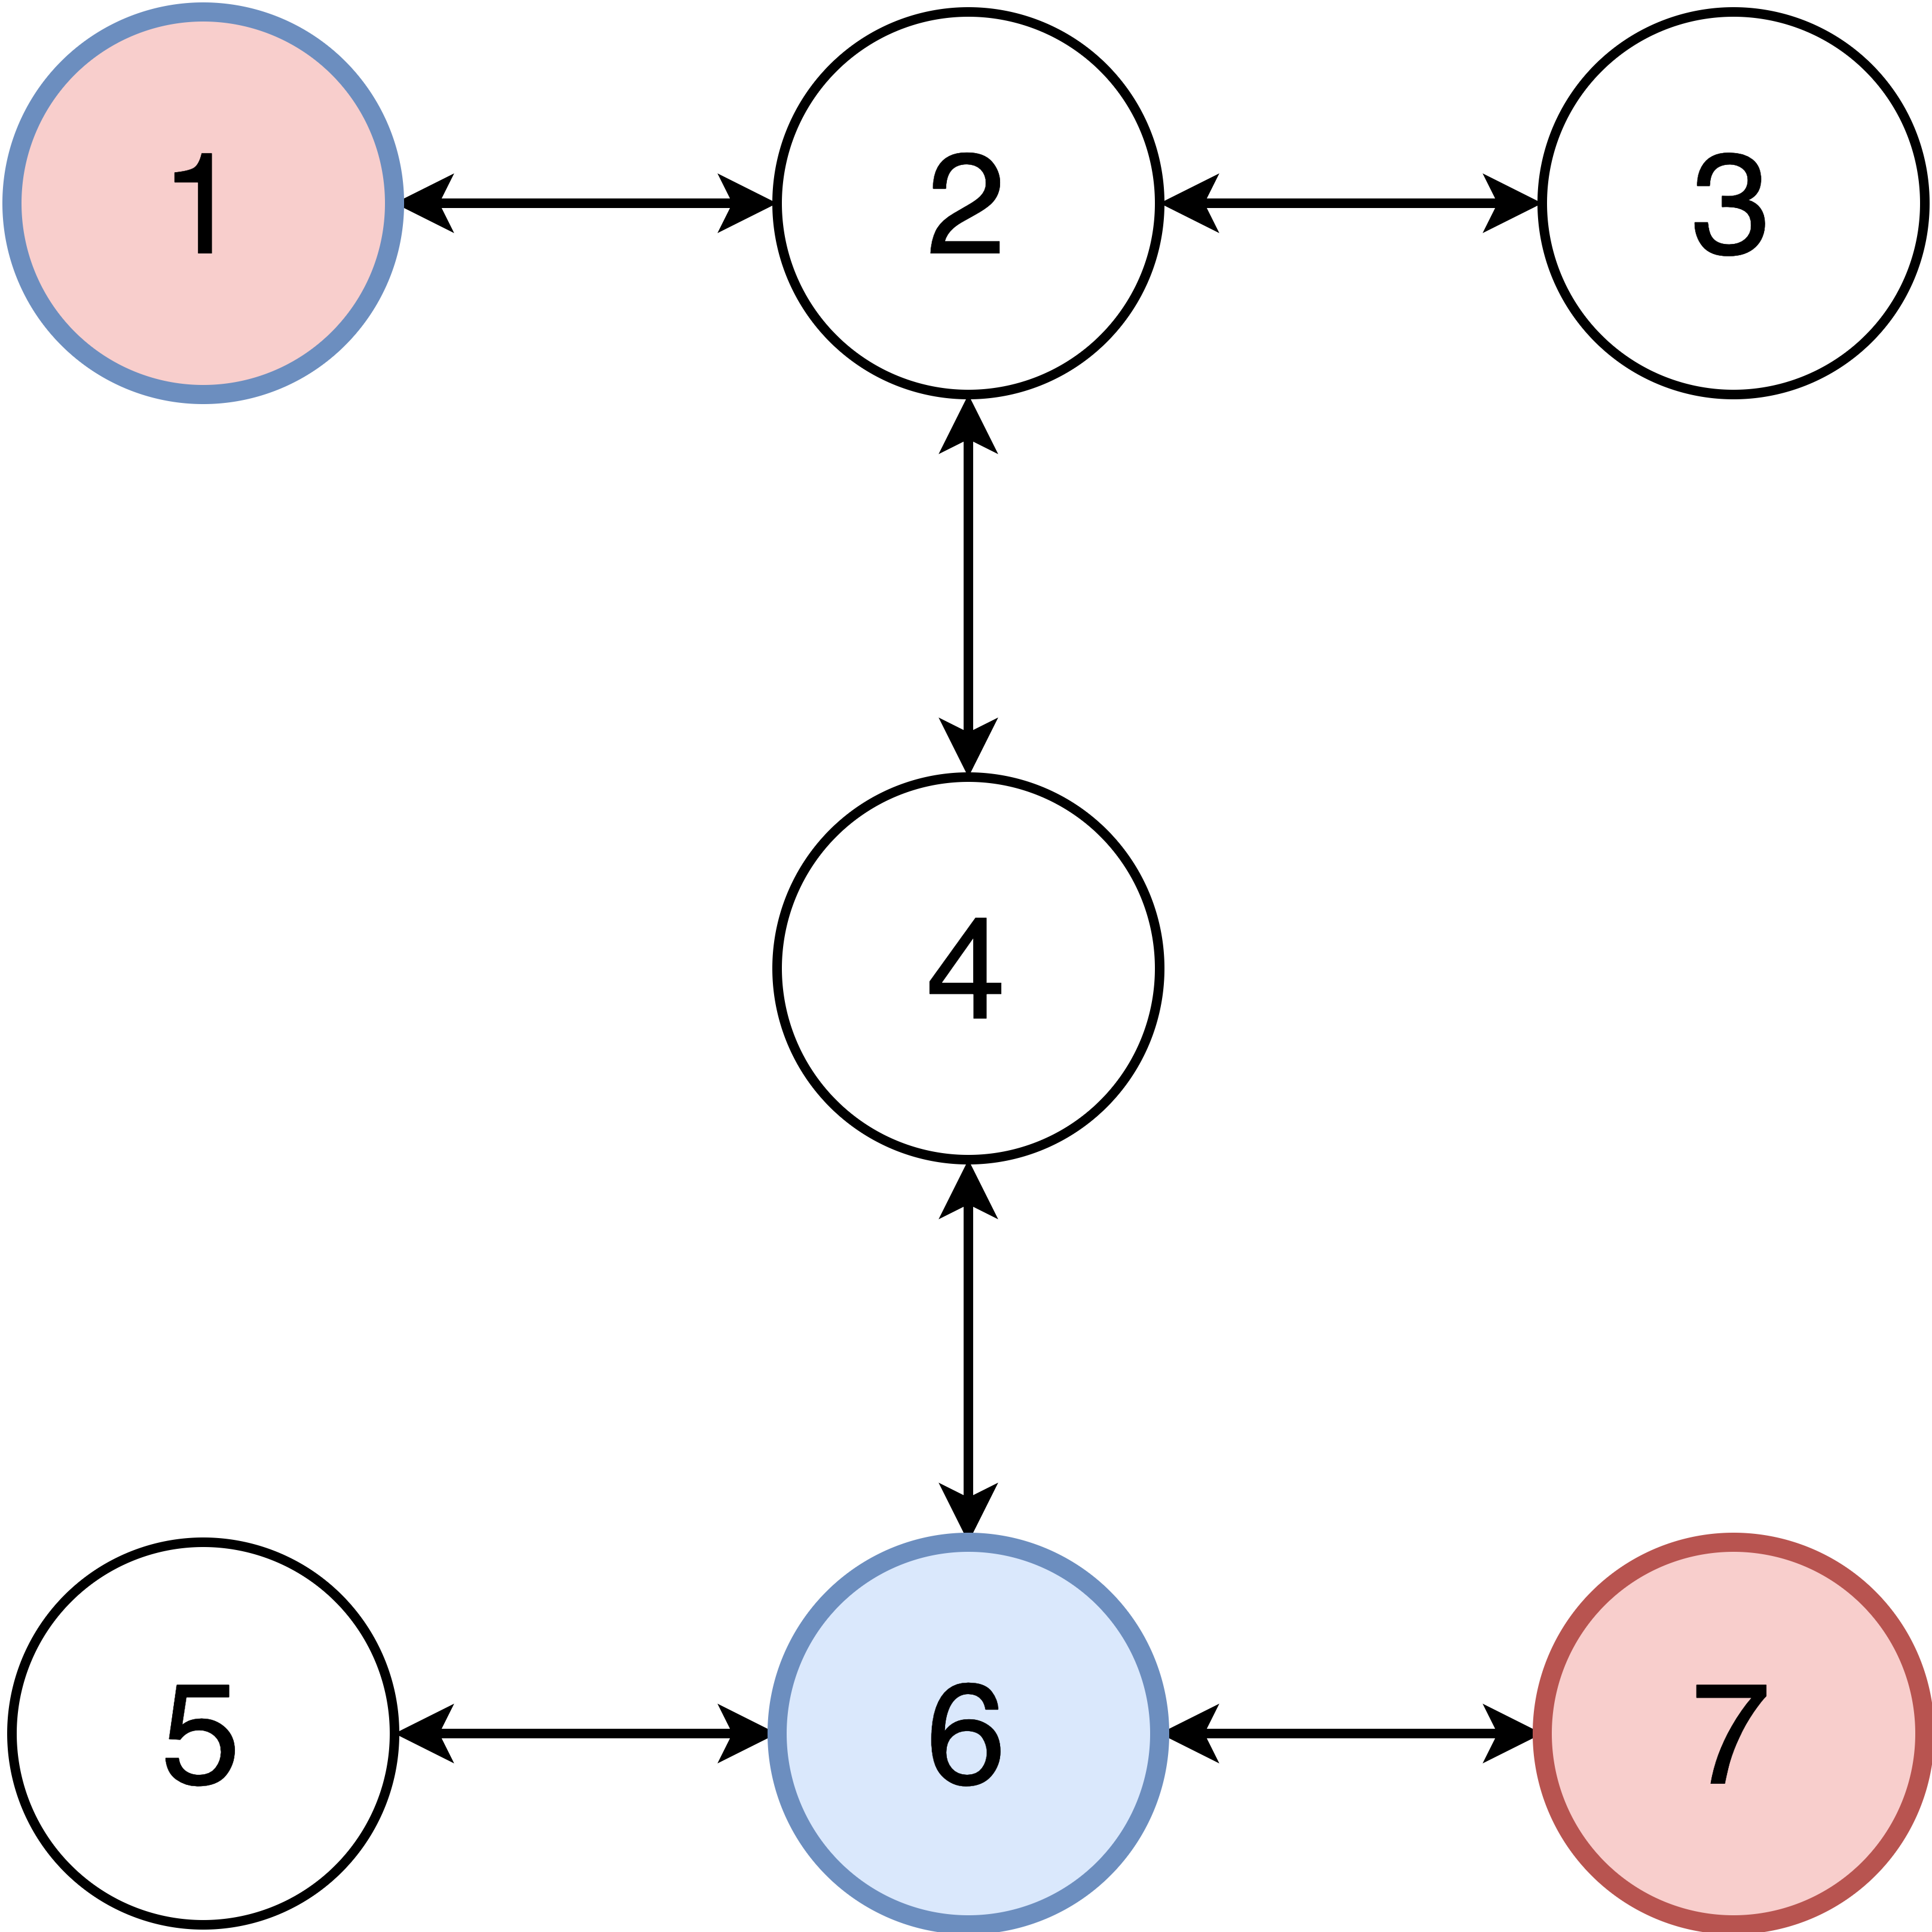
\includegraphics[width=0.35\textwidth]{swapProblem}
  \caption{A scenario which is not easily solvable with \acrs{CBS}. In blue are
  the initial (1) and final (6) nodes of hte first agent}
  \label{fig:swapProblem}
\end{figure}
By analyzing some of the failing cases we notice a pattern: each time two
agents follow the same shortest path in opposite directions and need to swap
places at an edge, the algorithms fail to efficiently solve the problem. An
example of this problem is shown in Figure~\ref{fig:swapProblem} where agent 1
(in blue) starts from node 1 and has to reach node 6, while agent 2 (in red)
starts from node 7 and has to reach node 1. In this case, the shortest paths,
and also only paths, to go from node 1 to 6 and from 7 to 1 are the following: 
\begin{minted}[linenos=false]{C}
1 : 1 2 4 6
2 : 7 6 4 2 1
\end{minted}
The problem is that none of the agents can wait on a node of the shortest path
without creating a conflict. The solution would be to consider additional nodes
that are not part of the shortest path, so that an agent could move aside
while the other freely passes. This is not something that is naturally done
by neither spanning trees nor shortest path algorithms, since it would require
to move twice on the same node. \newline
The idea to solve this problem in \acrs{TDSP} is similar to the idea of how
vertex conflicts have been handled so far, and that is by using a placeholder.
Indeed, at the moment the virtual nodes are used as a way to say to the
algorithm that the agents has to wait on a node to avoid a conflict, but they
may well be used as a way to tell the agent to move to a neighboring node and
then move back to the previous node. In this case, to avoid problem with the
shortest path algorithm, we could use two placeholder, one for the neighboring
node and one for the original node, which otherwise would not be considered.
This though raises the problem of how to choose the neighboring node: in the
test we have carried out, no good solution on this choice has been found. The
best solution would be to return a list of possible paths instead of a single
one, but this would also imply that the high-level search should carry multiple
paths weighing the process down. Indeed, it is not possible to say a priori
that choosing a neighbor instead of another is the best idea in terms of future
conflicts. \newline
Instead, the spanning tree algorithm may be improved by considering a counter
keeping track of how many times the algorithm has moved over some nodes. For
example, if we know that at time $t$ there would be a swap conflict between
node $n_1$ and node $n_2$, then we could let the algorithm move multiple times
over $n_1$, which would allow the neighboring nodes to be explored. \newline
This though is part of the future work on the \acrs{MAPF} aiming at creating a
framework for solving the problem with a wide range of possible algorithms. 
